\documentclass{article}
\usepackage{cmap}
\usepackage[utf8]{inputenc}
\usepackage[english,ukrainian]{babel}
\usepackage{graphicx}
\usepackage{geometry}
\usepackage{listings}
\usepackage{float}
\usepackage{amsmath}
\usepackage{subfig}
\usepackage{xcolor}
\geometry{
	a4paper,
	left=20mm,
	right=20mm,
	top=15mm,
	bottom=15mm,
}
\lstset{
	tabsize=4,
	keepspaces,
	showstringspaces=false,
	escapeinside={(*@}{@*)},
}
\graphicspath{ {./pictures} }
\setlength{\parindent}{4em}

\newcommand\subject{Архітектура комп'ютера}
\newcommand\lecturer{доцент кафедри ПЗ\\Крук О.Г.}
\newcommand\teacher{доцент кафедри ПЗ\\Крук О.Г.}
\newcommand\mygroup{ПЗ-22}
\newcommand\lab{6}
\newcommand\theme{Програмування арифметичного співпроцесора мікропроцесорів х86}
\newcommand\purpose{Розвинути навики складання програми для арифметичного співпроцесора мовою асемблера для обчислення математичного виразу, відтранслювати і виконати в режимі відлагодження програму, складену відповідно до свого варіанту, обчислити заданий вираз в програмі мовою С та порівняти результати}

\begin{document}
	\begin{normalsize}
		\begin{titlepage}
			\thispagestyle{empty}
			\begin{center}
				\textbf{МІНІСТЕРСТВО ОСВІТИ І НАУКИ УКРАЇНИ\\
					НАЦІОНАЛЬНИЙ УНІВЕРСИТЕТ "ЛЬВІВСЬКА ПОЛІТЕХНІКА"}
			\end{center}
			\begin{flushright}
				\textbf{ІКНІ}\\
				Кафедра \textbf{ПЗ}
			\end{flushright}
			\vspace{200pt}
			\begin{center}
				\textbf{ЗВІТ}\\
				\vspace{10pt}
				до лабораторної роботи № \lab\\
				\textbf{на тему}: “\textit{\theme}”\\
				\textbf{з дисципліни}: “\subject”
			\end{center}
			\vspace{112pt}
			\begin{flushright}
				
				\textbf{Лектор}:\\
				\lecturer\\
				\vspace{28pt}
				\textbf{Виконав}:\\
				
				студент групи \mygroup\\
				Коваленко Д.М.\\
				\vspace{28pt}
				\textbf{Прийняв}:\\
				
				\teacher\\
				
				\vspace{28pt}
				«\rule{1cm}{0.15mm}» \rule{1.5cm}{0.15mm} 2022 р.\\
				$\sum$ = \rule{1cm}{0.15mm}……………\\
				
			\end{flushright}
			\vspace{\fill}
			\begin{center}
				\textbf{Львів — 2022}
			\end{center}
		\end{titlepage}
		
		\begin{description}
			\item[Тема.] \theme.
			\item[Мета.] \purpose.
		\end{description}
		
		\section*{Індивідуальне завдання}
		\begin{figure}[H]
			\centering
			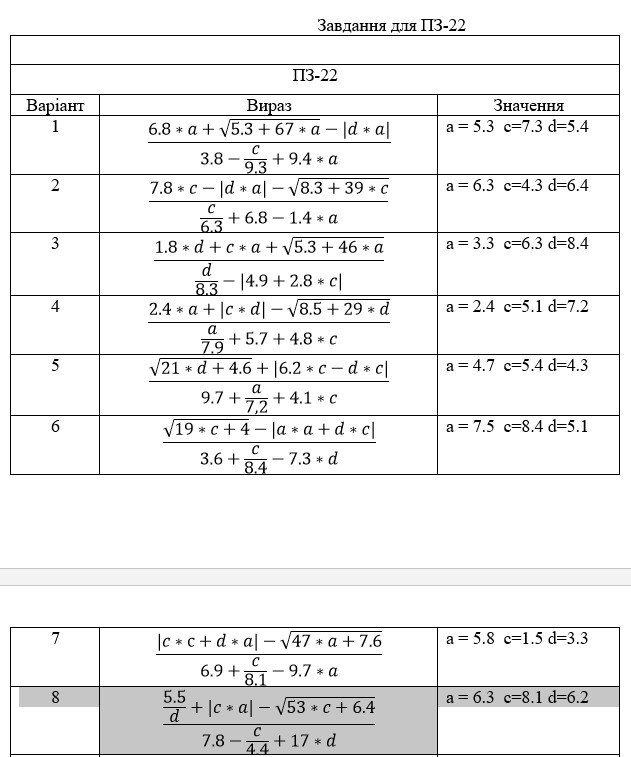
\includegraphics[scale=0.6]{v}
		\end{figure}
		
		\section*{Хід роботи}
		Вираз у зворотньому польському записі:
		\begin{gather}
			\text{TOP:} \hspace{5pt}5.5\text{ D }/\text{ C A }* abs + 53\text{ C }* 6.4 + sqrt -\nonumber\\
			\text{BOT:} \hspace{83pt}7.8\text{ C }4.4 / -  17\text{ D }* +\nonumber\\
			\text{RES:} \hspace{130pt}\text{TOP BOT} /\nonumber
		\end{gather}
		\subsection*{Код програми (Асемблер)}
		\begin{lstlisting}[language={[x86masm]Assembler}]
			.686 
			.model flat,stdcall 
			.stack 
			
			.data 
			
			A REAL4 6.3
			B REAL4 8.1; C
			D REAL4 6.2
			C1 REAL4 5.5
			C2 REAL4 53.0
			C3 REAL4 6.4
			C4 REAL4 7.8
			C5 REAL4 4.4
			C6 REAL4 17.0
			
			TOP REAL4 ? 
			BOT REAL4 ? 
			
			RES REAL4 ? 
			
			.code 
			main: 
			finit 
			fld  C1    ; 5.5/D
			fdiv D
			
			fld B	    ; |C*A|
			fmul A
			fabs
			
			faddp 
			
			fld  C2    ; sqrt(53*C+6.4)
			fmul B
			fadd C3 
			fsqrt 
			
			fsubp 
			fst TOP
			
			fld  C4    ; 7.8
			
			fld  B    ; C/4.4
			fdiv C5 
			
			fsubp
			
			fld  C6    ; 17*D
			fmul D
			
			faddp
			fst BOT 
			
			fld TOP 
			fdiv BOT 
			fst RES 
			
			RET 
			END main
		\end{lstlisting}
		
		\begin{figure}[H]
			\centering
			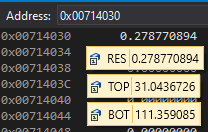
\includegraphics[scale=1]{1}
			\caption{Результат виконання програми}
		\end{figure}
		
		\subsection*{Код програми (C)}
		\begin{lstlisting}[language={C}]
			#include <stdio.h>
			#include <stdlib.h>
			#include <math.h>
			
			int main() {
				float a = 6.3, c = 8.1, d = 6.2;
				
				float top = (5.5/d) + abs(c*a) - sqrt(53.0*c + 6.4);
				float bot = 7.8 - (c/4.4) + 17.0*d;
				float res = top/bot;
				printf("%f\n", top);
				printf("%f\n", bot);
				printf("%f\n", res);
			}
			
		\end{lstlisting}
		
		\begin{figure}[H]
			\centering
			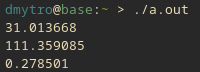
\includegraphics[scale=1]{2}
			\caption{Результат виконання програми}
		\end{figure}
		
		\section*{Висновки}
		Під час виконання лабораторної роботи я розвинув навики складання програми для арифметичного співпроцесора мовою асемблера для обчислення математичного виразу, відтранслював і виконав в режимі відлагодження програму, складену відповідно до свого варіанту, обчислив заданий вираз в програмі мовою С та порівняти результати.
		
	\end{normalsize}
\end{document}